\documentclass{beamer}

\usepackage{Freifunkstil}
\usepackage[]{ulem}
\usepackage[font=small,skip=0pt]{caption}
\usepackage[extendedchars]{grffile}
\captionsetup{font=scriptsize,labelfont=scriptsize}
\setbeamertemplate{mini frames}{}
\begin{document}
\title{Freifunk}
\subtitle{Freies WLAN für alle}
\author[I. Otter, M. Walther]{Ingomar Otter, Matthias Walther}
\date{27.07.2016\\\vspace{0.3cm} 
\includegraphics[scale=0.3]{Vorlagen/logo-transparent.png}}
\institute{Freifunk Münsterland\\Förderverein freie Infrastruktur e. V.}

\begin{frame}
\titlepage	
\end{frame}
\begin{frame}{Inhaltsverzeichnis}
	\tableofcontents
\end{frame}
\section{Ziele von Freifunk}
\begin{frame}{Freifunk aus Sicht des Routeraufstellers}
	Freifunk ermöglicht es jedem Mitmachenden sein Internet zu teilen und den Menschen in seiner Umgebung freies WLAN anzubieten. Die Prinzipien dabei sind:
	\begin{itemize}
		\item WLAN für Gäste, Kunden oder Passanten in der Umgebung
		\item niedrige Kosten
		\item Jeder kann mitmachen
		\item Dezentralität
		\item Erweiterbarkeit des Netzes
		\item Rechtssicherheit
	\end{itemize}
\end{frame}
\begin{frame}{Freifunk aus Sicht des Nutzers}
	\begin{itemize}
		\item Freies und kostenloses WLAN möglichst überall, vorzugsweise in Innenstädten
		\item niedrige Einstiegshürde für Nutzer
			\begin{itemize}
				\item keine Vorschaltseite
				\item kein Passwort
				\item Barrierefreiheit
			\end{itemize}
		\item Keine Zeit- oder Volumenbegrenzung für den Nutzer
		\item Roaming, also Wechsel des Accesspoints ohne Neuanmeldung meines Geräts
		\item Keine technischen Einschränkungen
			\begin{itemize}
				\item keine Portsperren
				\item keine Inhaltefilter
				\item Netzneutralität
			\end{itemize}
		\item Automatische Verbindung bei zukünftigen Besuchen
	\end{itemize}
\end{frame}
\section{Technische Abwicklung}
\begin{frame}{Wie kann ich Freifunk nutzen?}
	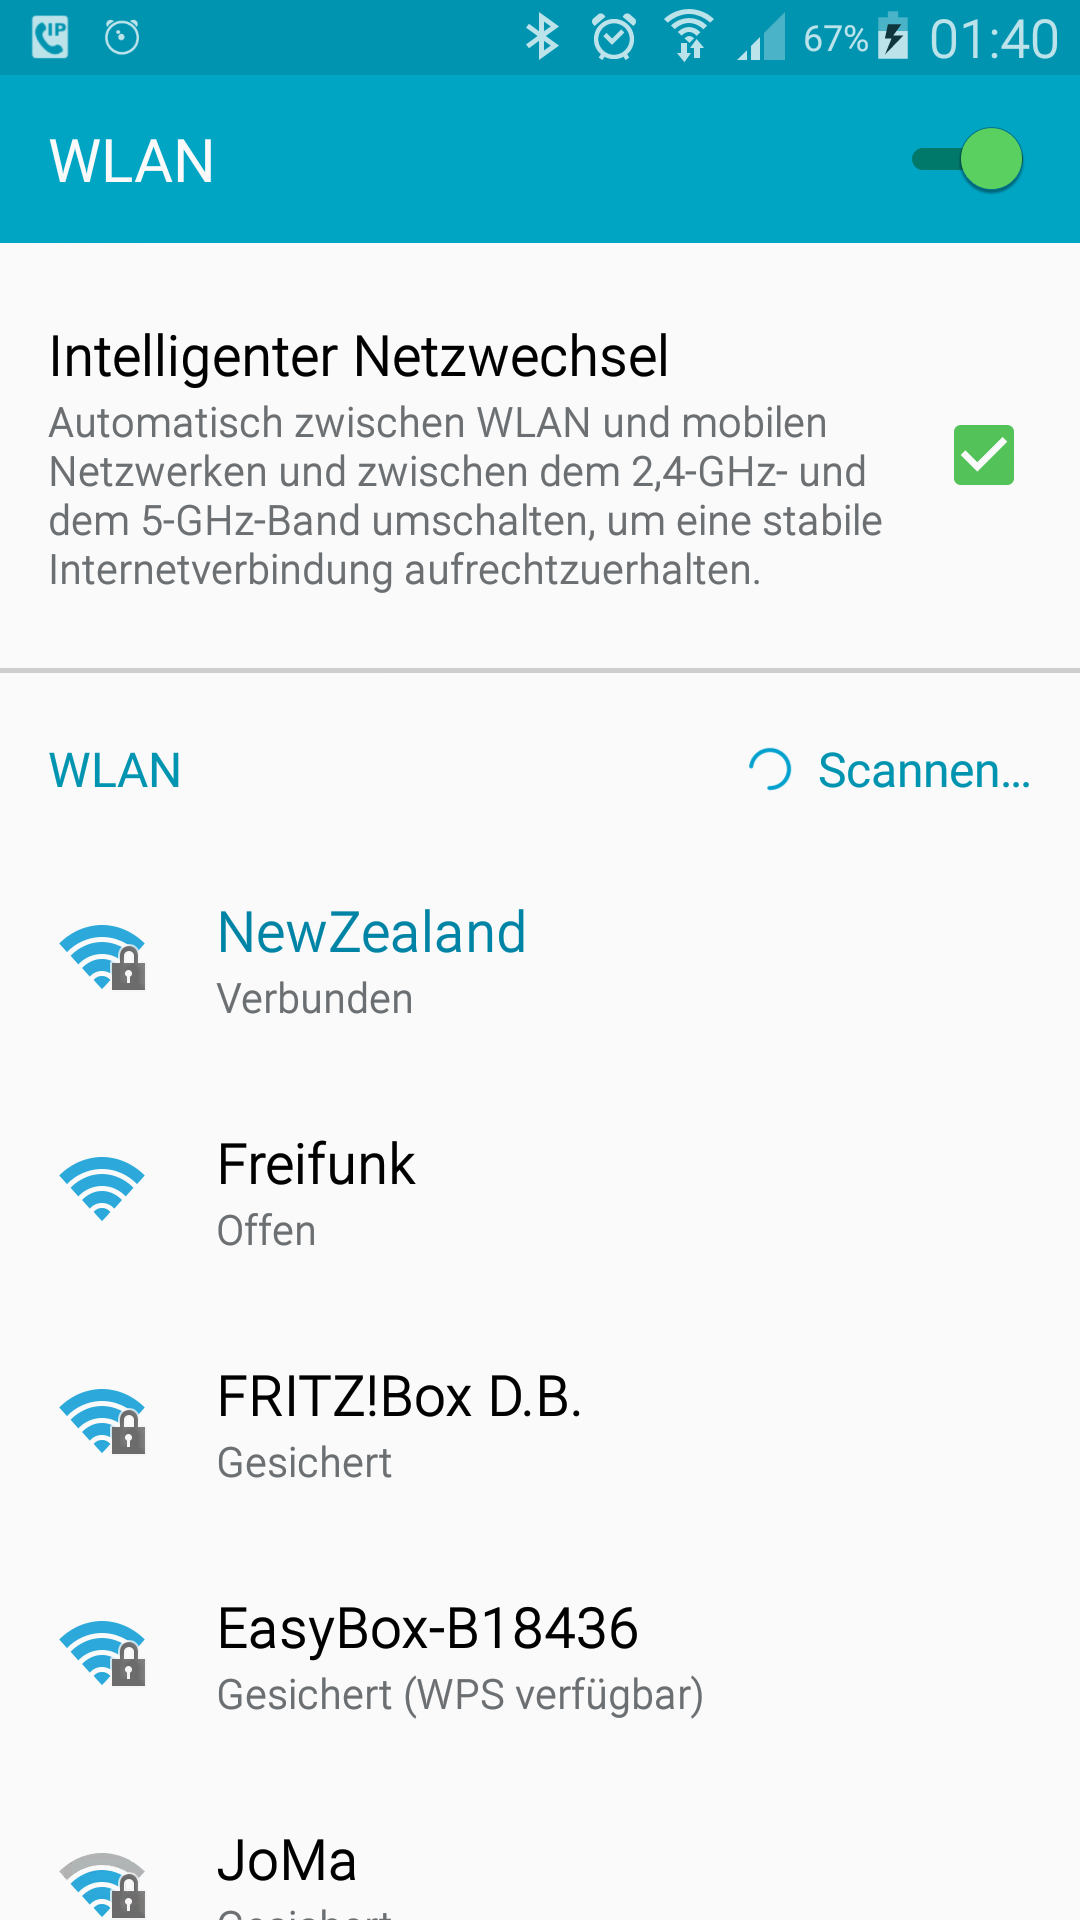
\includegraphics[width=0.25\textwidth]{verbinden0.png}
	\hspace*{0.5mm}
	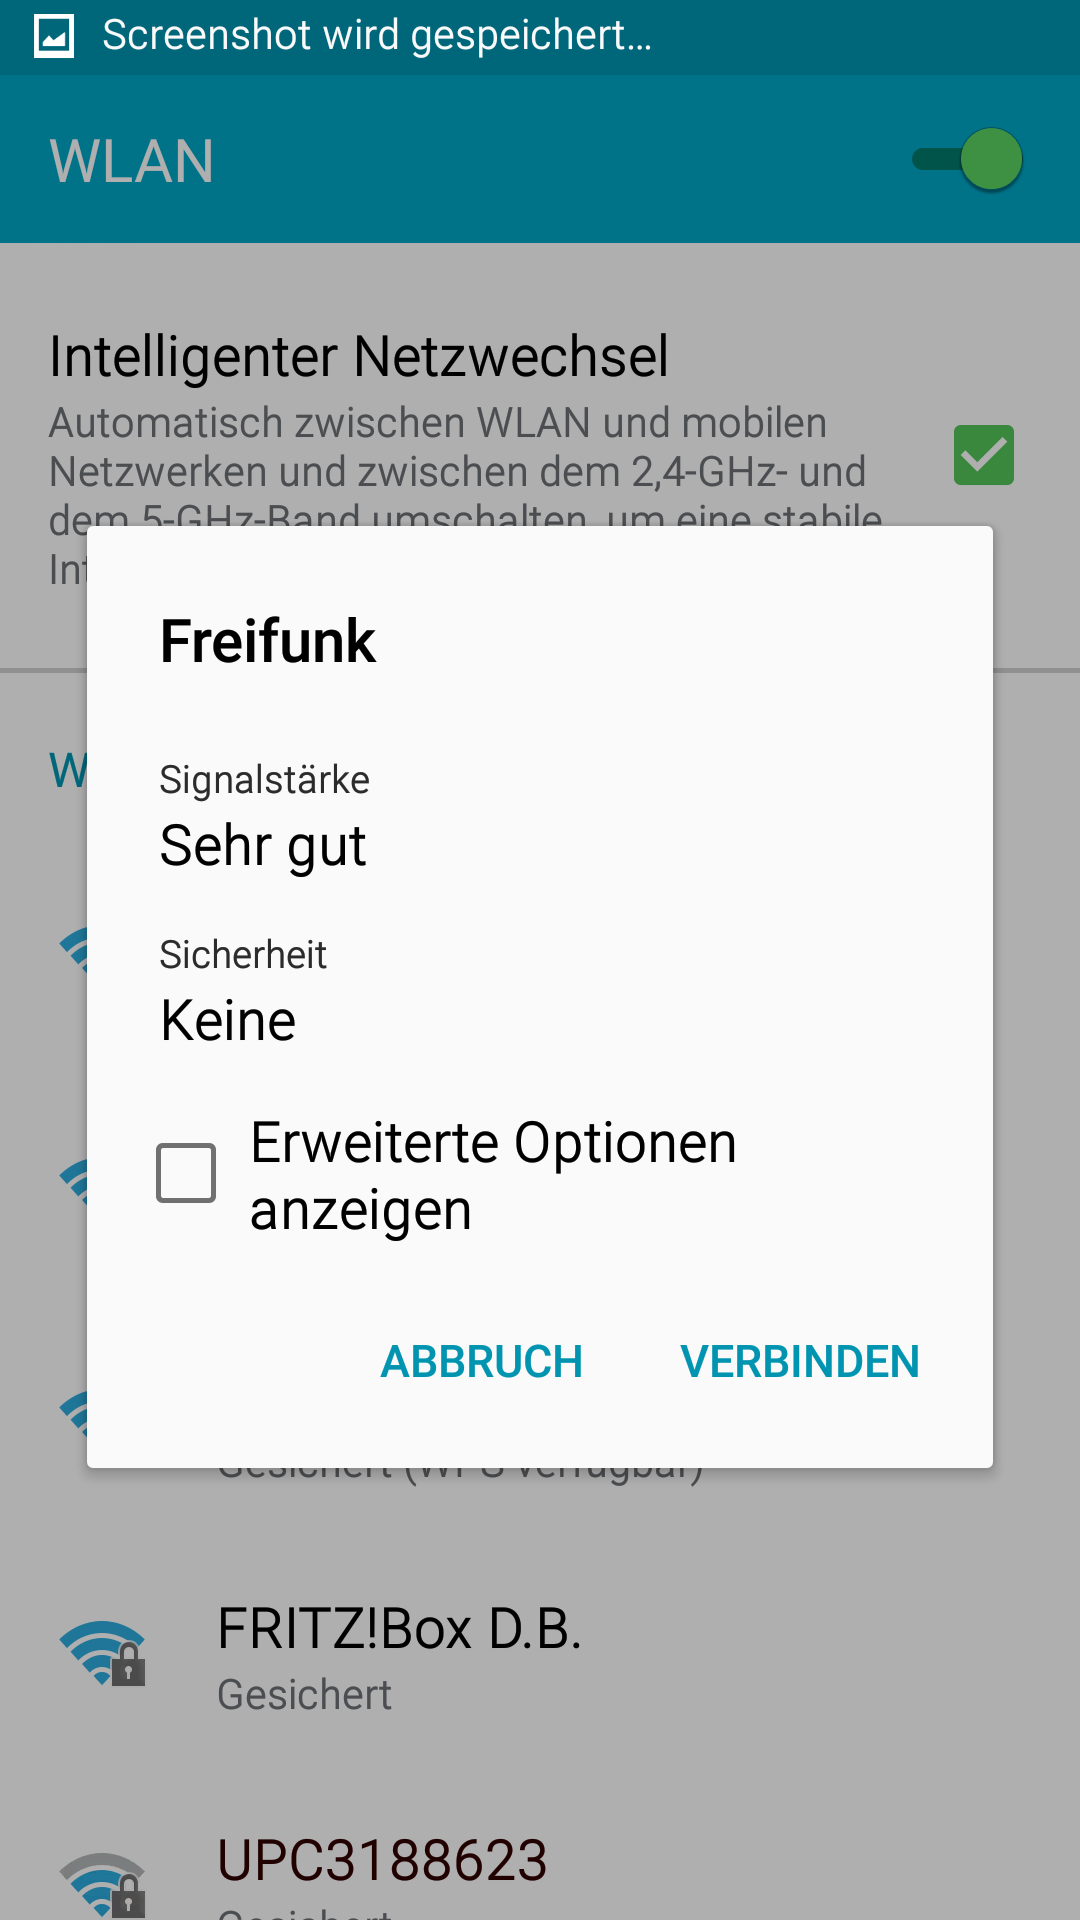
\includegraphics[width=0.25\textwidth]{verbinden1.png}
	\hspace*{0.5mm}
	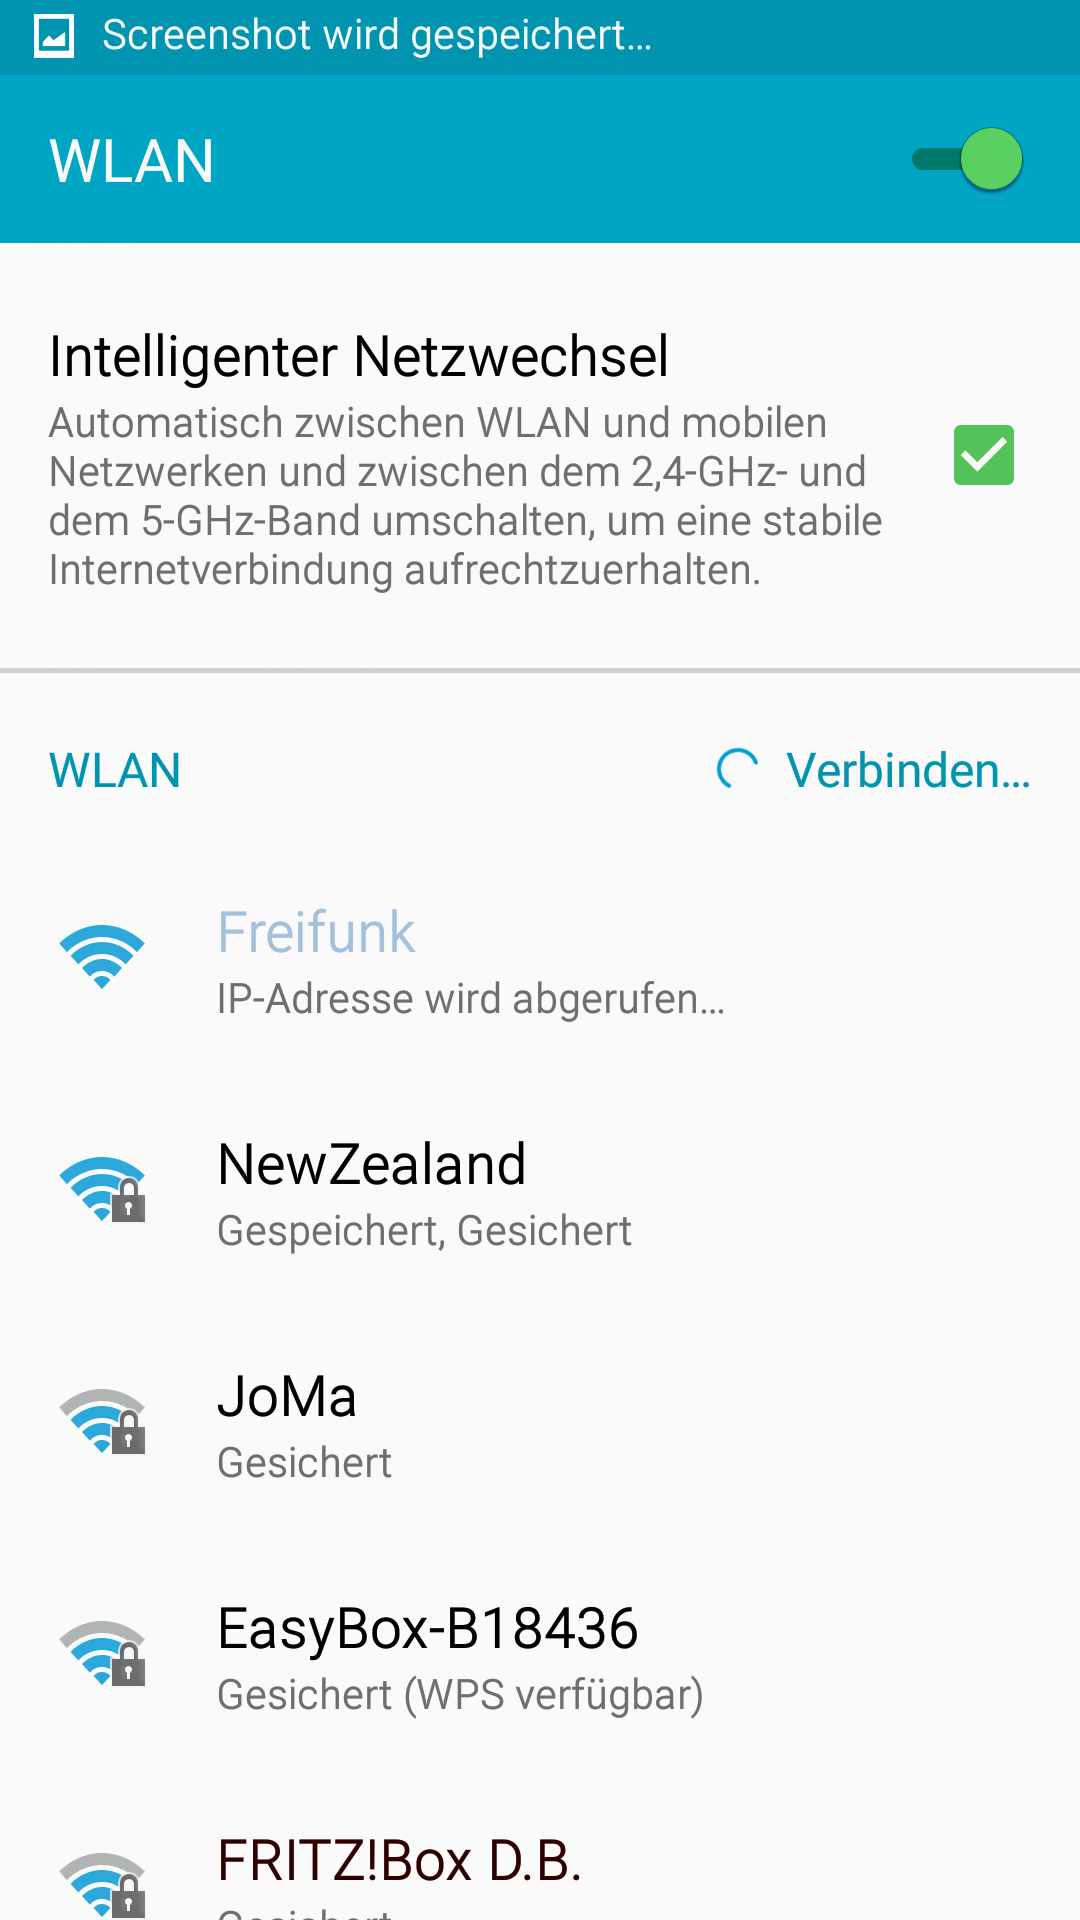
\includegraphics[width=0.25\textwidth]{verbinden2.png}
	\hspace*{0.5mm}
	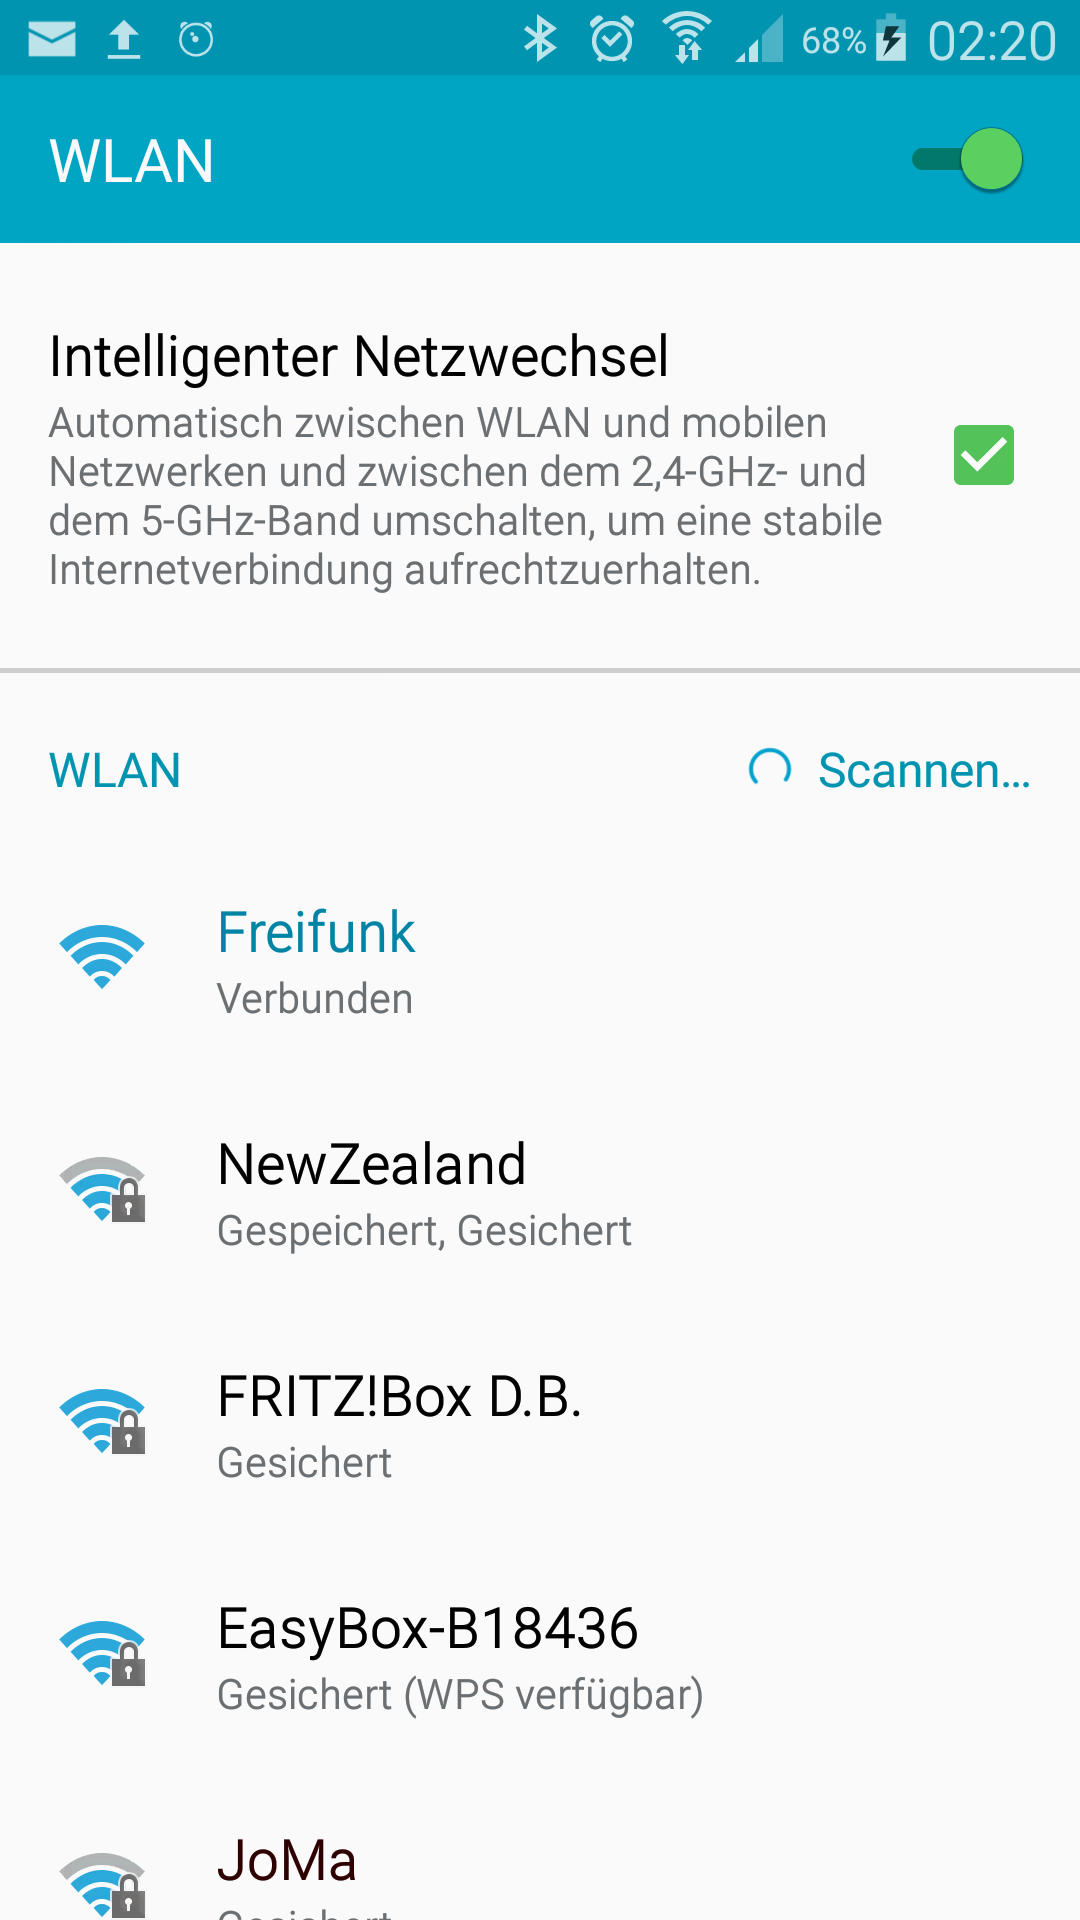
\includegraphics[width=0.25\textwidth]{verbinden3.png}
	
\end{frame}
\begin{frame}{Erweiterbarkeit durch Vermaschung (Mesh)}
	\hspace*{-11.0mm}
	\includegraphics<1>[width=\paperwidth,keepaspectratio]{mesh0}
	\includegraphics<2>[width=\paperwidth,keepaspectratio]{mesh1}
	\includegraphics<3>[width=\paperwidth,keepaspectratio]{mesh2}
	\includegraphics<4>[width=\paperwidth,keepaspectratio]{mesh3}
	
\end{frame}
\begin{frame}{Beispiel Rorup}
	\begin{center}
	\vspace*{-1.1mm}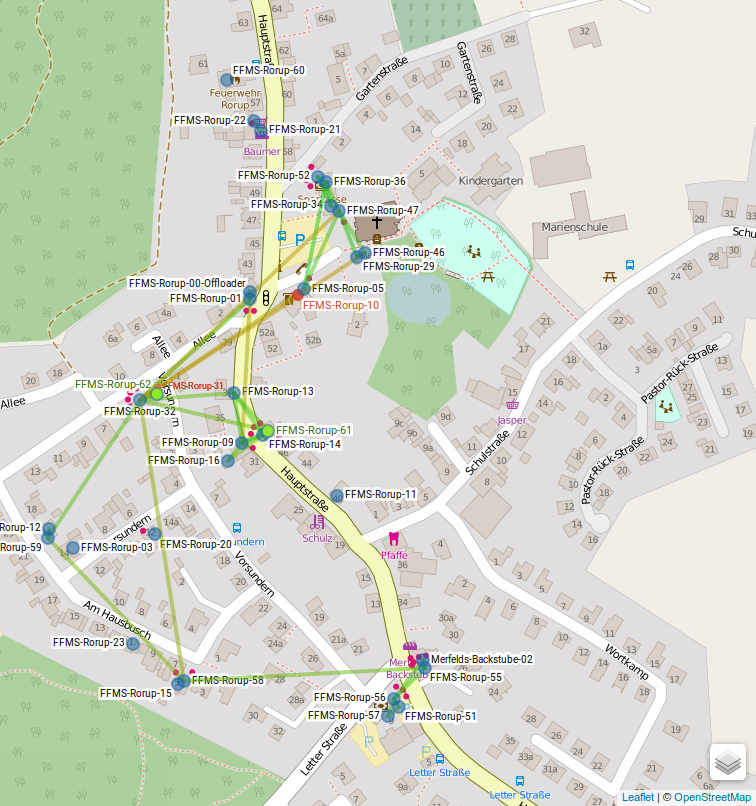
\includegraphics[height=0.8\textheight,keepaspectratio]{rorup-mesch.png}
\end{center}
\end{frame}
\subsection{Störerhaftung}
\begin{frame}{Netzaufbau}
	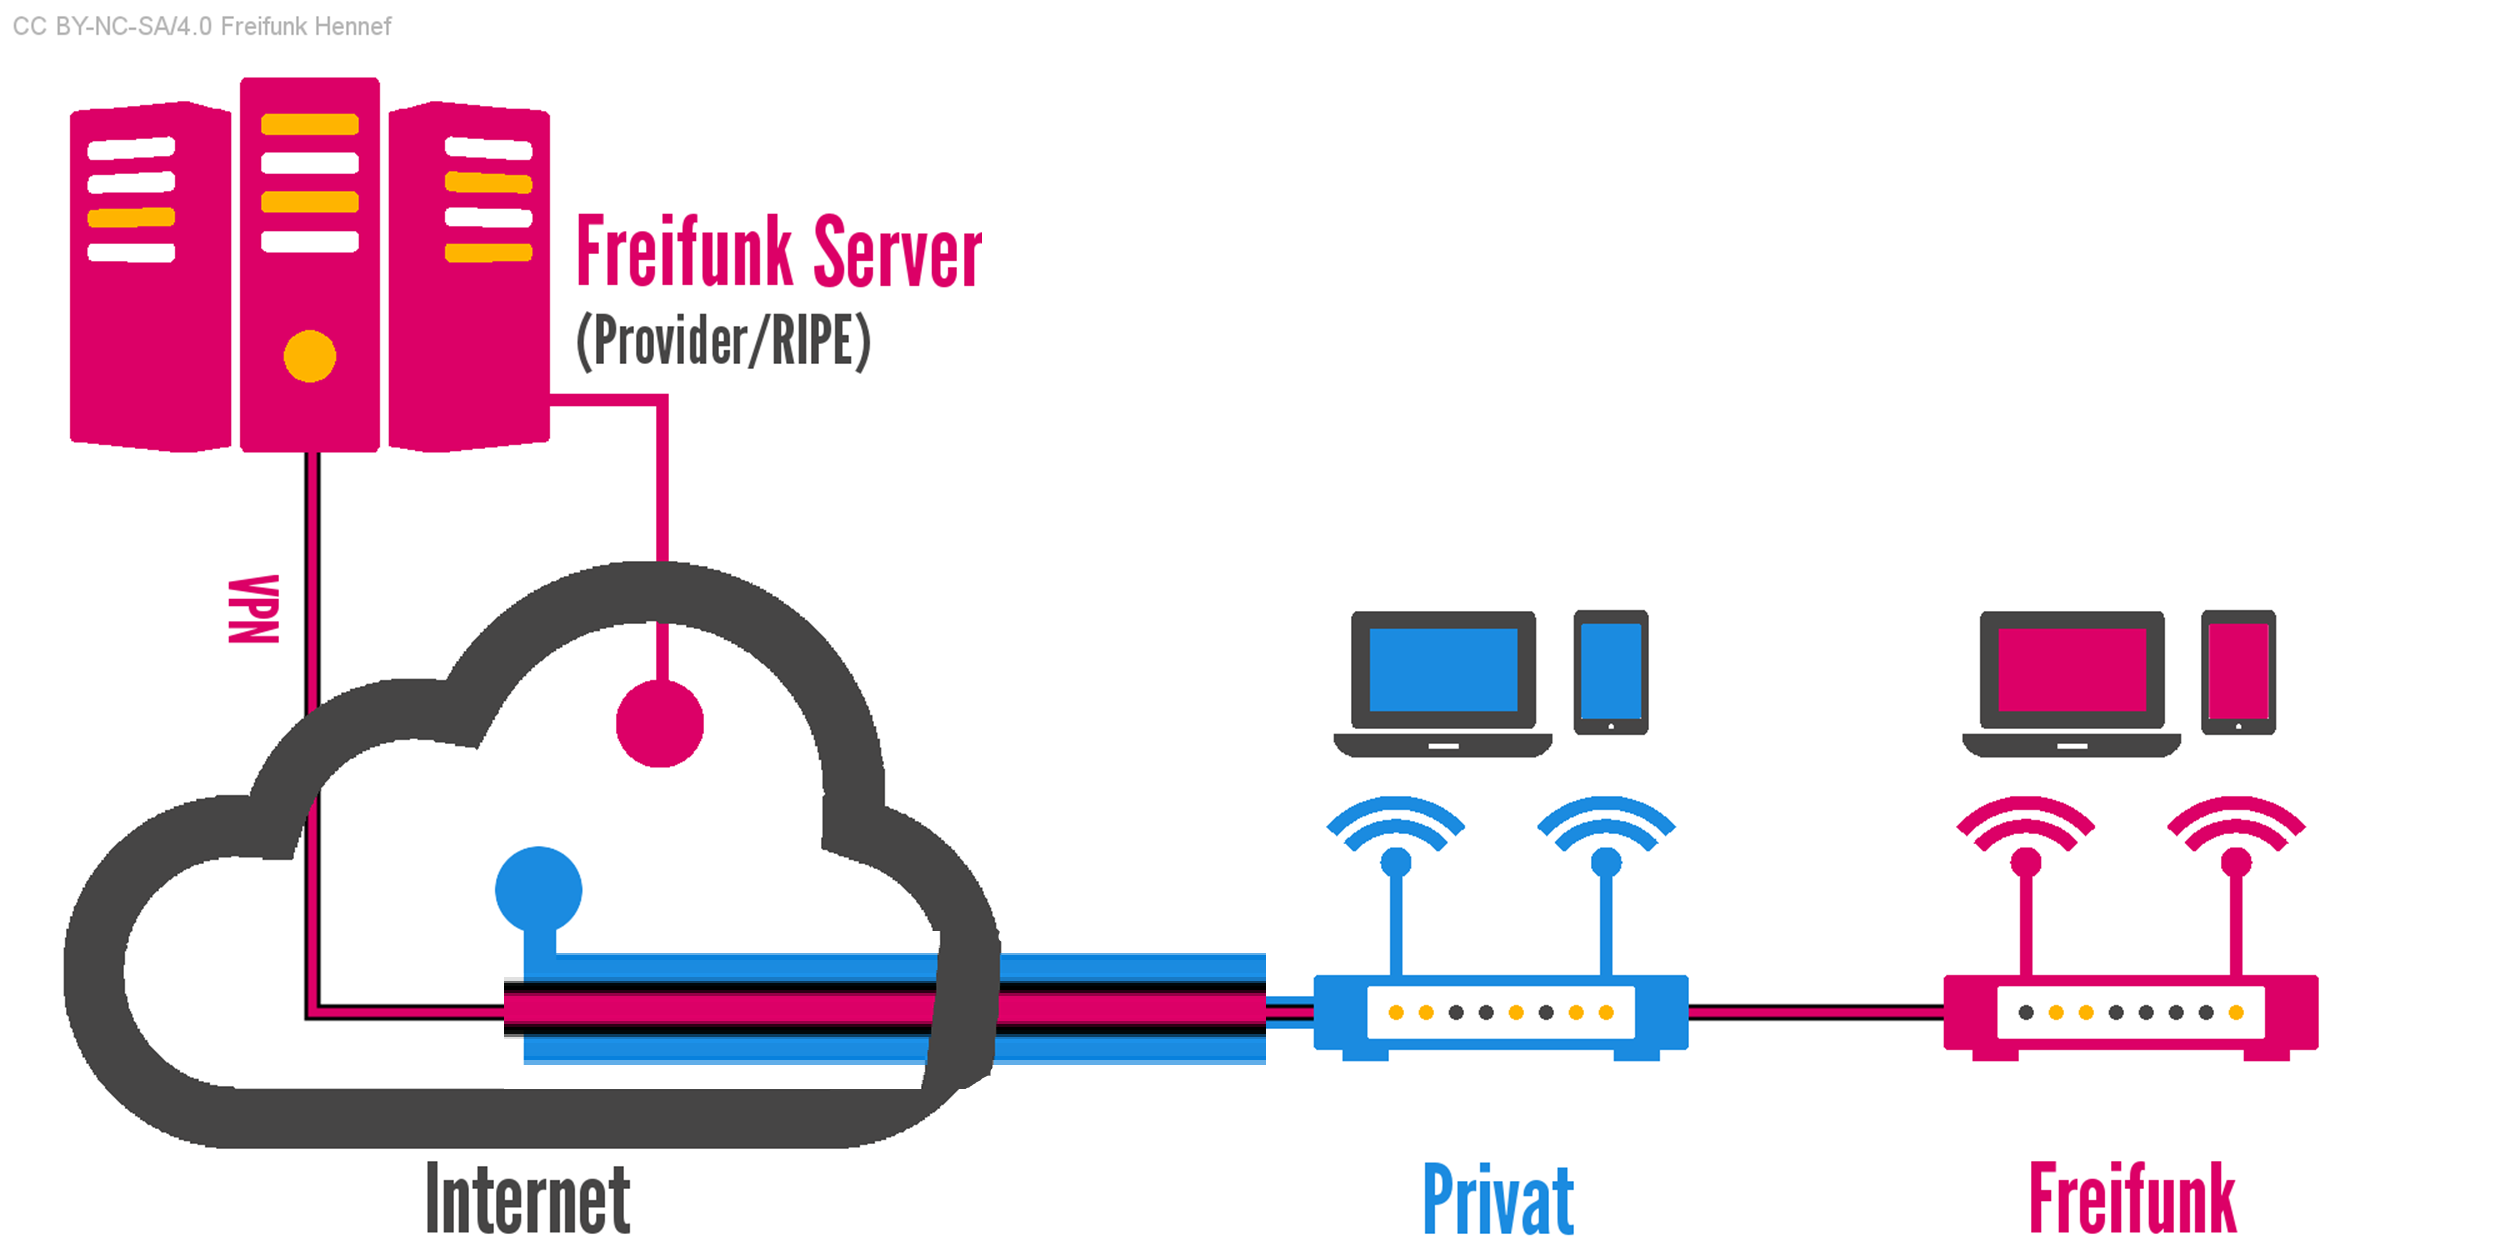
\includegraphics[height=0.9\textheight,width=\textwidth,keepaspectratio]{Netzskizze.png}
\end{frame}
\begin{frame}{Störerhaftung}
	\begin{itemize}
		\item Jegliche Internetzugriffe werden durch das VPN erst zu den Freifunkservern umgeleitet und dort erst ins Internet geleitet
		\item bewirkt eine Änderung der IP-Adresse
		\item IP-Adresse des Knotenaufstellers von außen nicht sichtbar
		\item Eventuelle Missbrauchsfälle landen bei Freifunk, nicht beim Knotenbetreiber
		\item keine Abmahnungen
		\item Technisch selbes Prinzip wie kommerzielle Anbieter
	\end{itemize}
\end{frame}
\section{Wie kann ich mitmachen?}
\begin{frame}
	\begin{enumerate}
		\item Privatperson / Geschäftsinhaber
		\item Förderung durch Werbegemeinschaften oder Banken
		\item Gemeinde
	\end{enumerate}
\end{frame}
\subsection{Privatperson / Geschäftsinhaber}
\begin{frame}
	\begin{columns}
		\begin{column}{0.4\textwidth}
			\begin{center}
			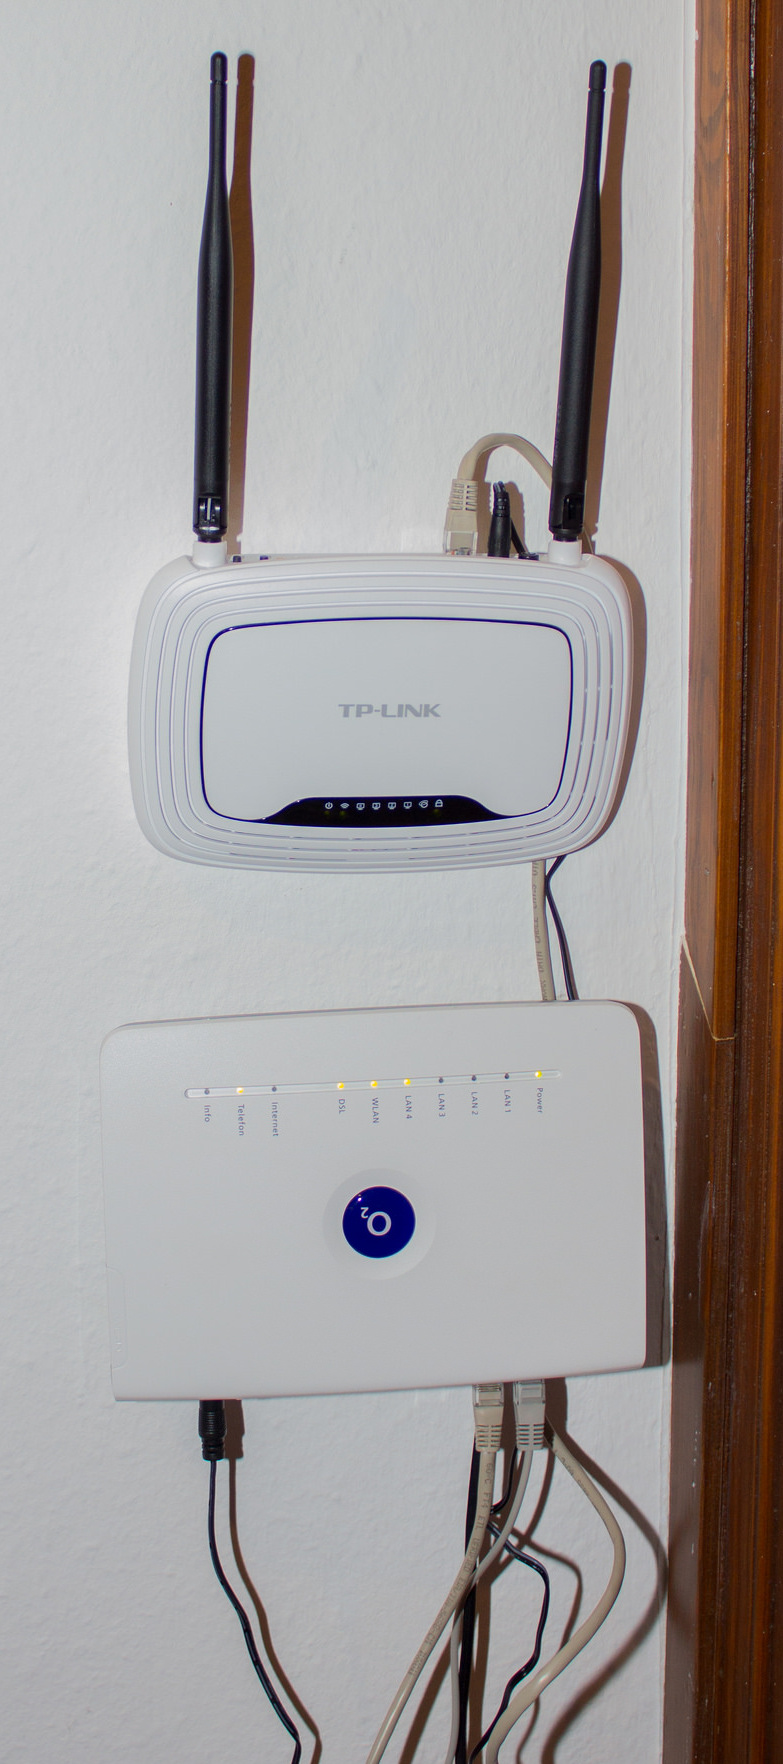
\includegraphics[height=0.9\textheight,keepaspectratio]{freifunk-o2.jpg}\\
			\textit{\tiny CC-BY-NC Timo Schmitt}
		\end{center}
		\end{column}
		\begin{column}{0.5\textwidth}
			\begin{itemize}
				\item Internetanschluss möglichst ohne Volumenbegrenzung
				\item Freifunk-Router kaufen, mit Freifunksoftware bespielen und an den DSL/Kabel-Router anschließen
				\item Falls Freifunkrouter in der Nachbarschaft ggfs. reiner Meshrouter möglich
			\end{itemize}
		\end{column}
	\end{columns}
\end{frame}
\begin{frame}{Geräteauswahl}
	\begin{columns}
		\begin{column}{0.45\textwidth}
			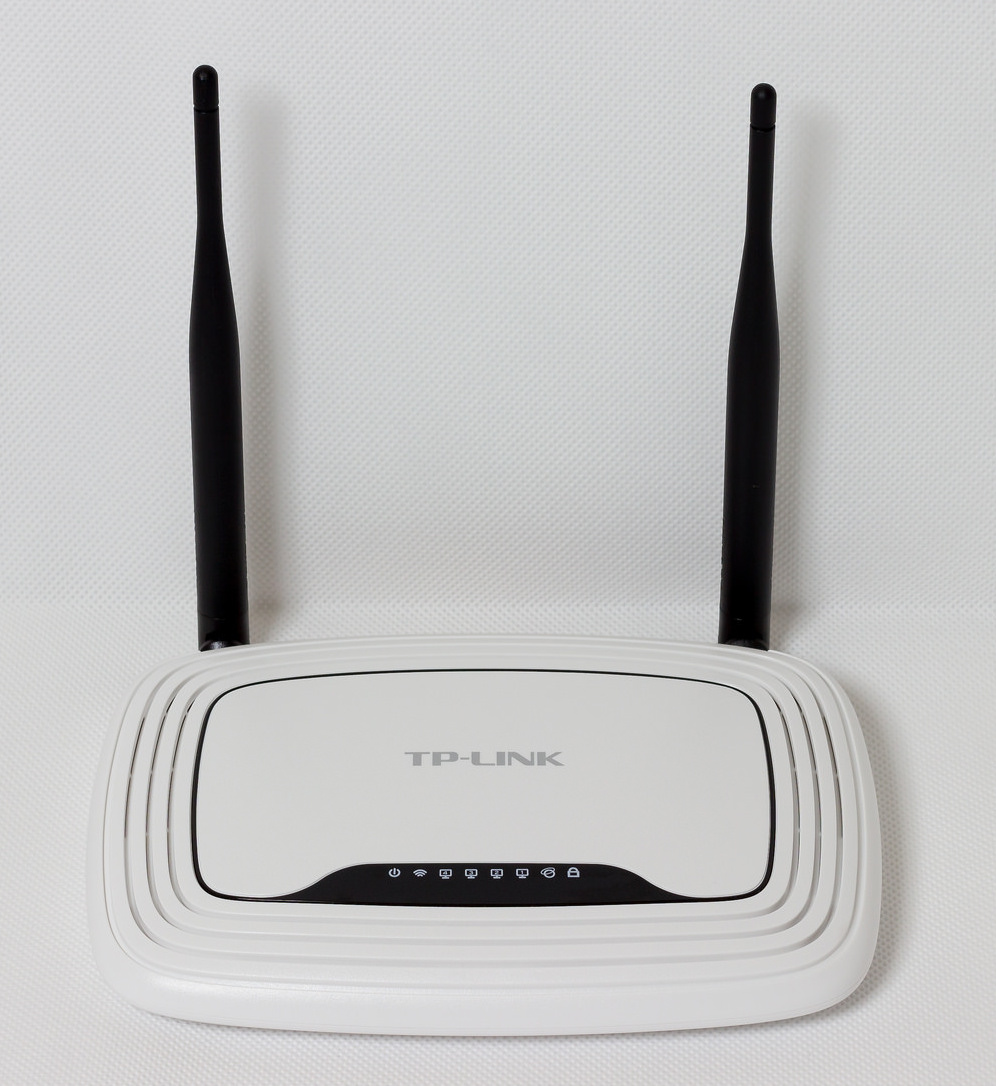
\includegraphics[height=0.5\textheight,keepaspectratio]{wr841n.jpg}\\
			\vspace*{-2.0mm}\textit{\tiny TP-Link WR841N, CC-BY-NC Timo Schmitt}
			\begin{itemize}
				\item Standardgerät ab 20 \euro
				\item Für preissensible Installationen
			\end{itemize}

			
		\end{column}
		\begin{column}{0.45\textwidth}
			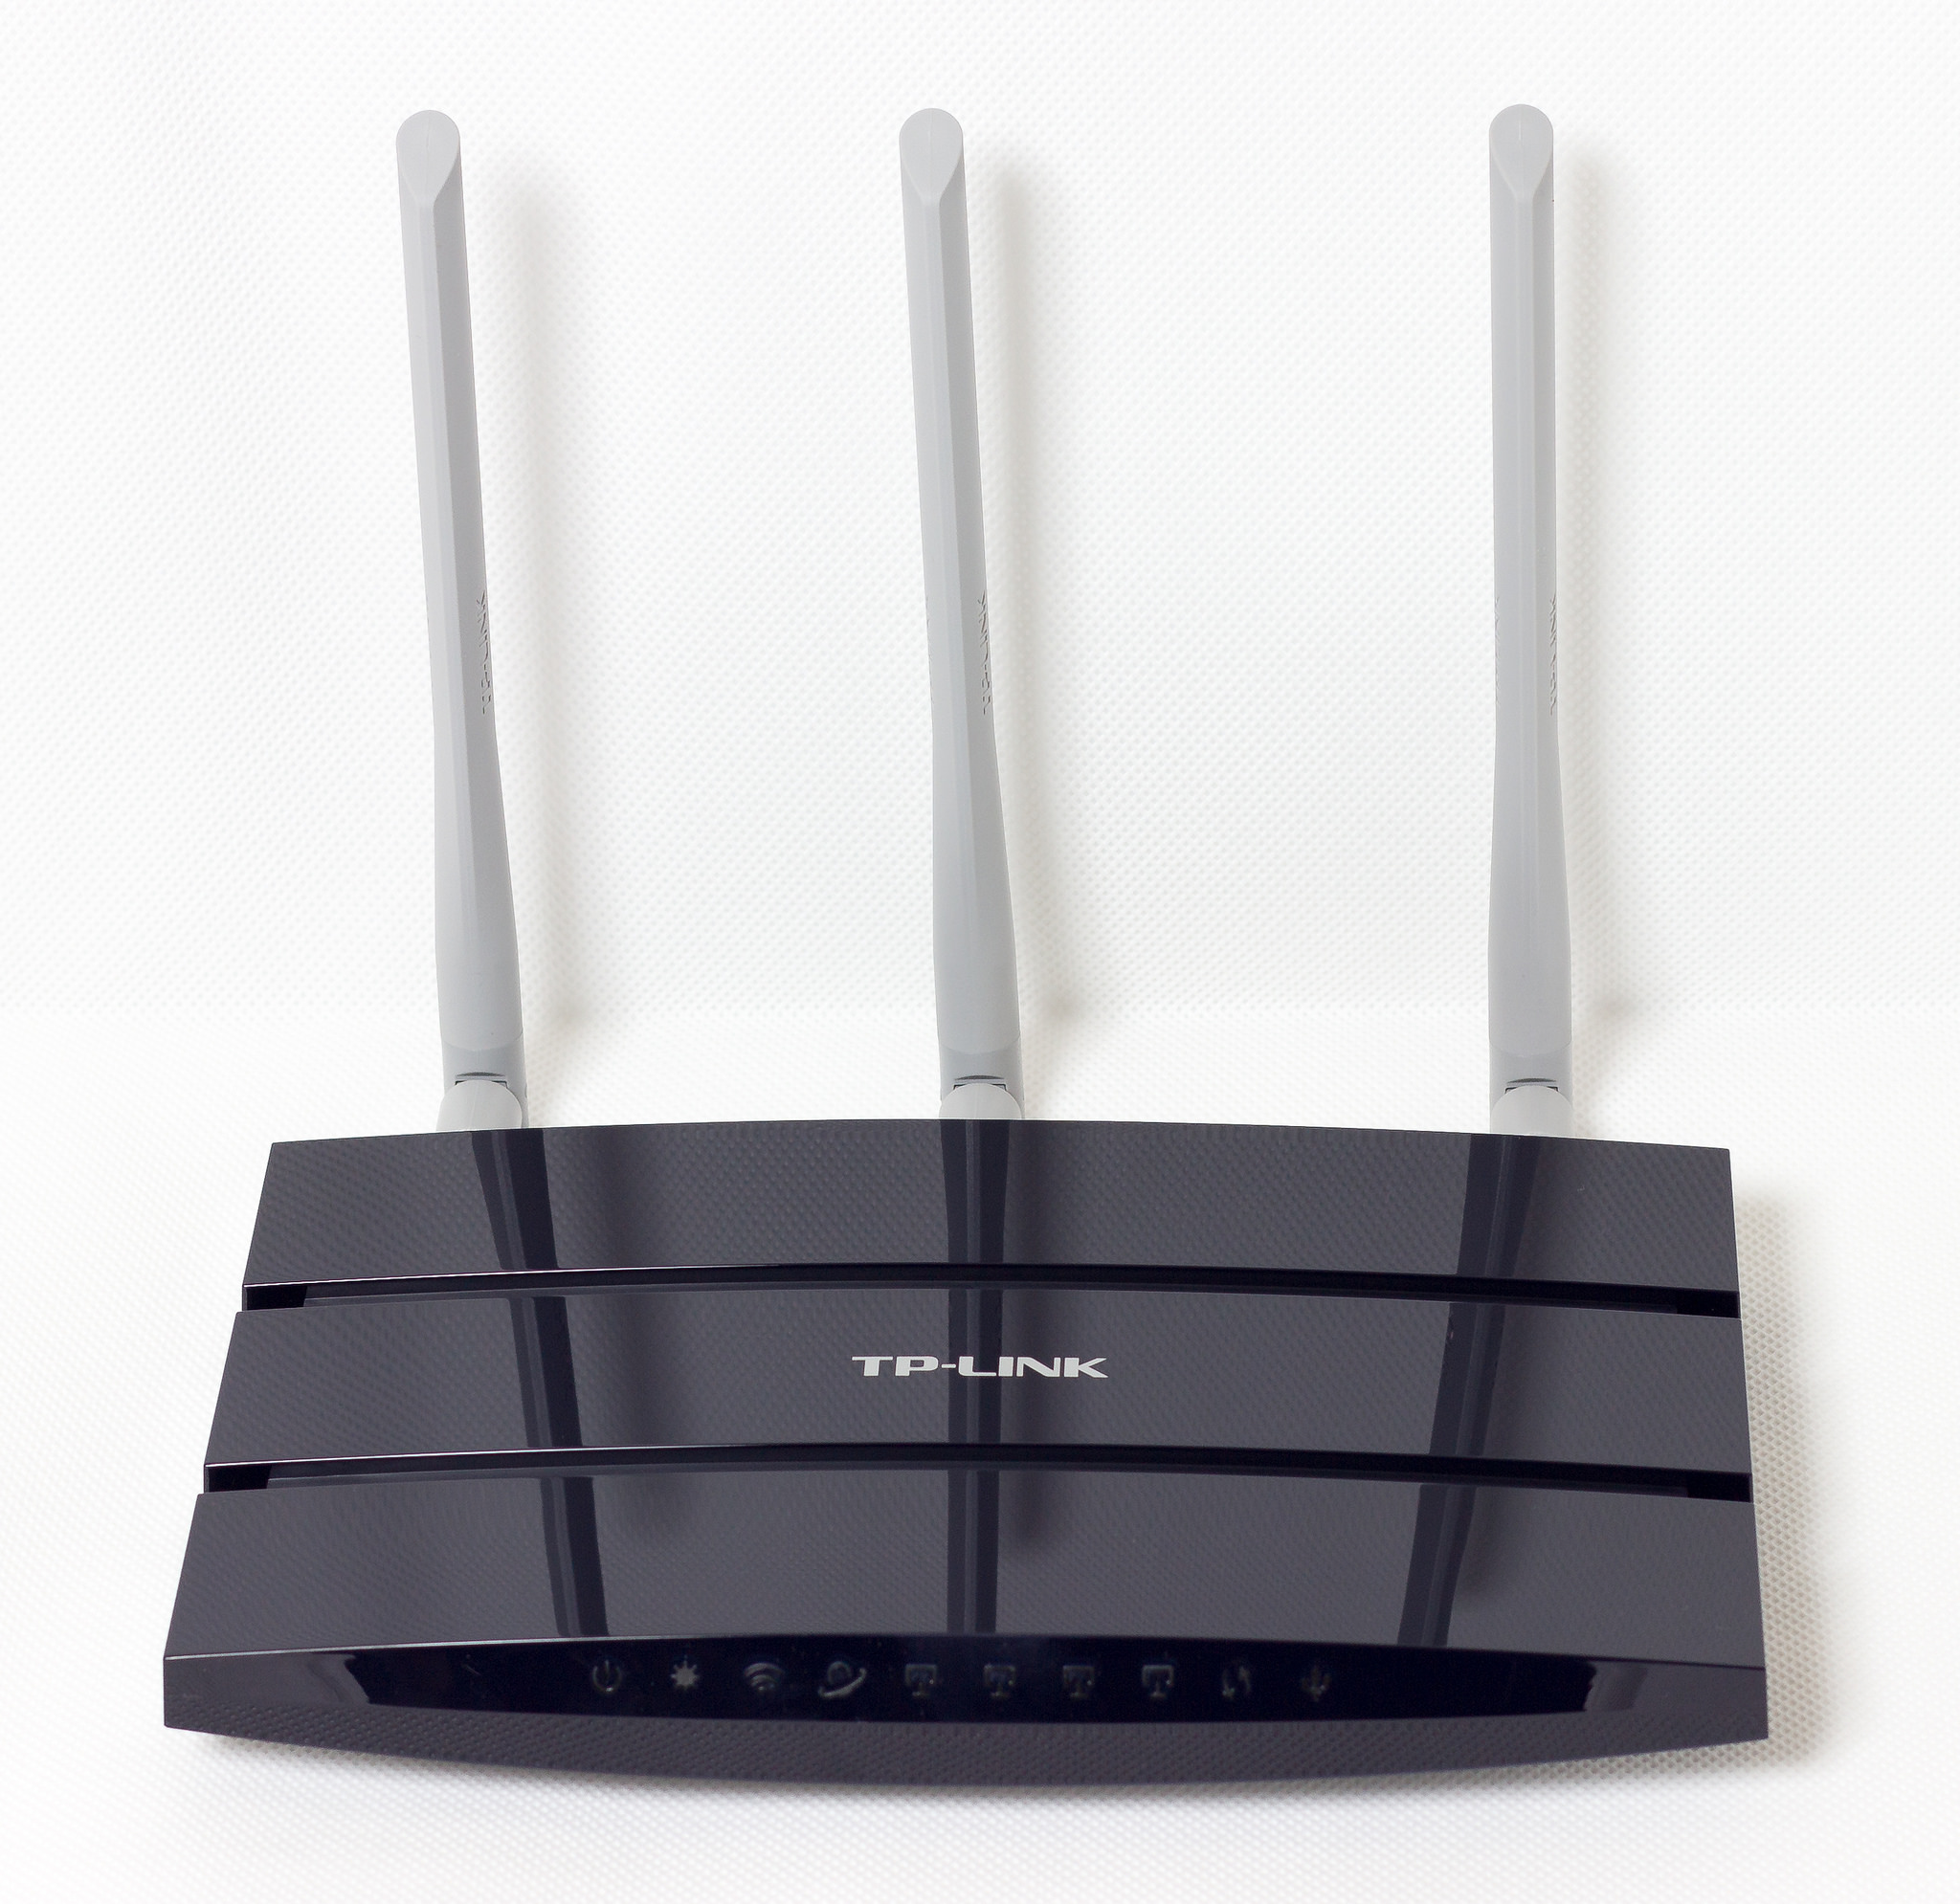
\includegraphics[height=0.5\textheight,keepaspectratio]{wr1043nd.jpg}\\
			\vspace*{-2.0mm}\textit{\tiny TP-Link WR1043ND, CC-BY-NC Timo Schmitt}
			\begin{itemize}
				\item Schafft mehr Clients 
				\item Ab etwa 50 \euro
				\item Empfehlung für Geschäfte
			\end{itemize}
			
		\end{column}
	\end{columns}
\end{frame}
\begin{frame}
	\begin{itemize}
		\item Gerät kann selbst gekauft und installiert werden
		\item Unterstützung durch Community, Forum und Ticketsystem
		\item oder Systemhaus beauftragen
	\end{itemize}
\end{frame}
\subsection{Werbegemeinschaften und Banken als Sponsoren}
\begin{frame}
	\begin{itemize}
		\item Unterstützung bei der Finanzierung von Außengeräten
	\end{itemize}
	\begin{columns}
		\begin{column}{0.45\textwidth}
			
\includegraphics[height=0.5\textheight,keepaspectratio]{cpe210.jpg}\\
			\vspace*{-2.0mm}\textit{\tiny TP-Link CPE210, CC-BY-NC Timo Schmitt}
			\begin{itemize}
				\item Sektorantenne 
				\item ab 50 \euro
				\item Außengerät
			\end{itemize}

			
		\end{column}
		\begin{column}{0.45\textwidth}
			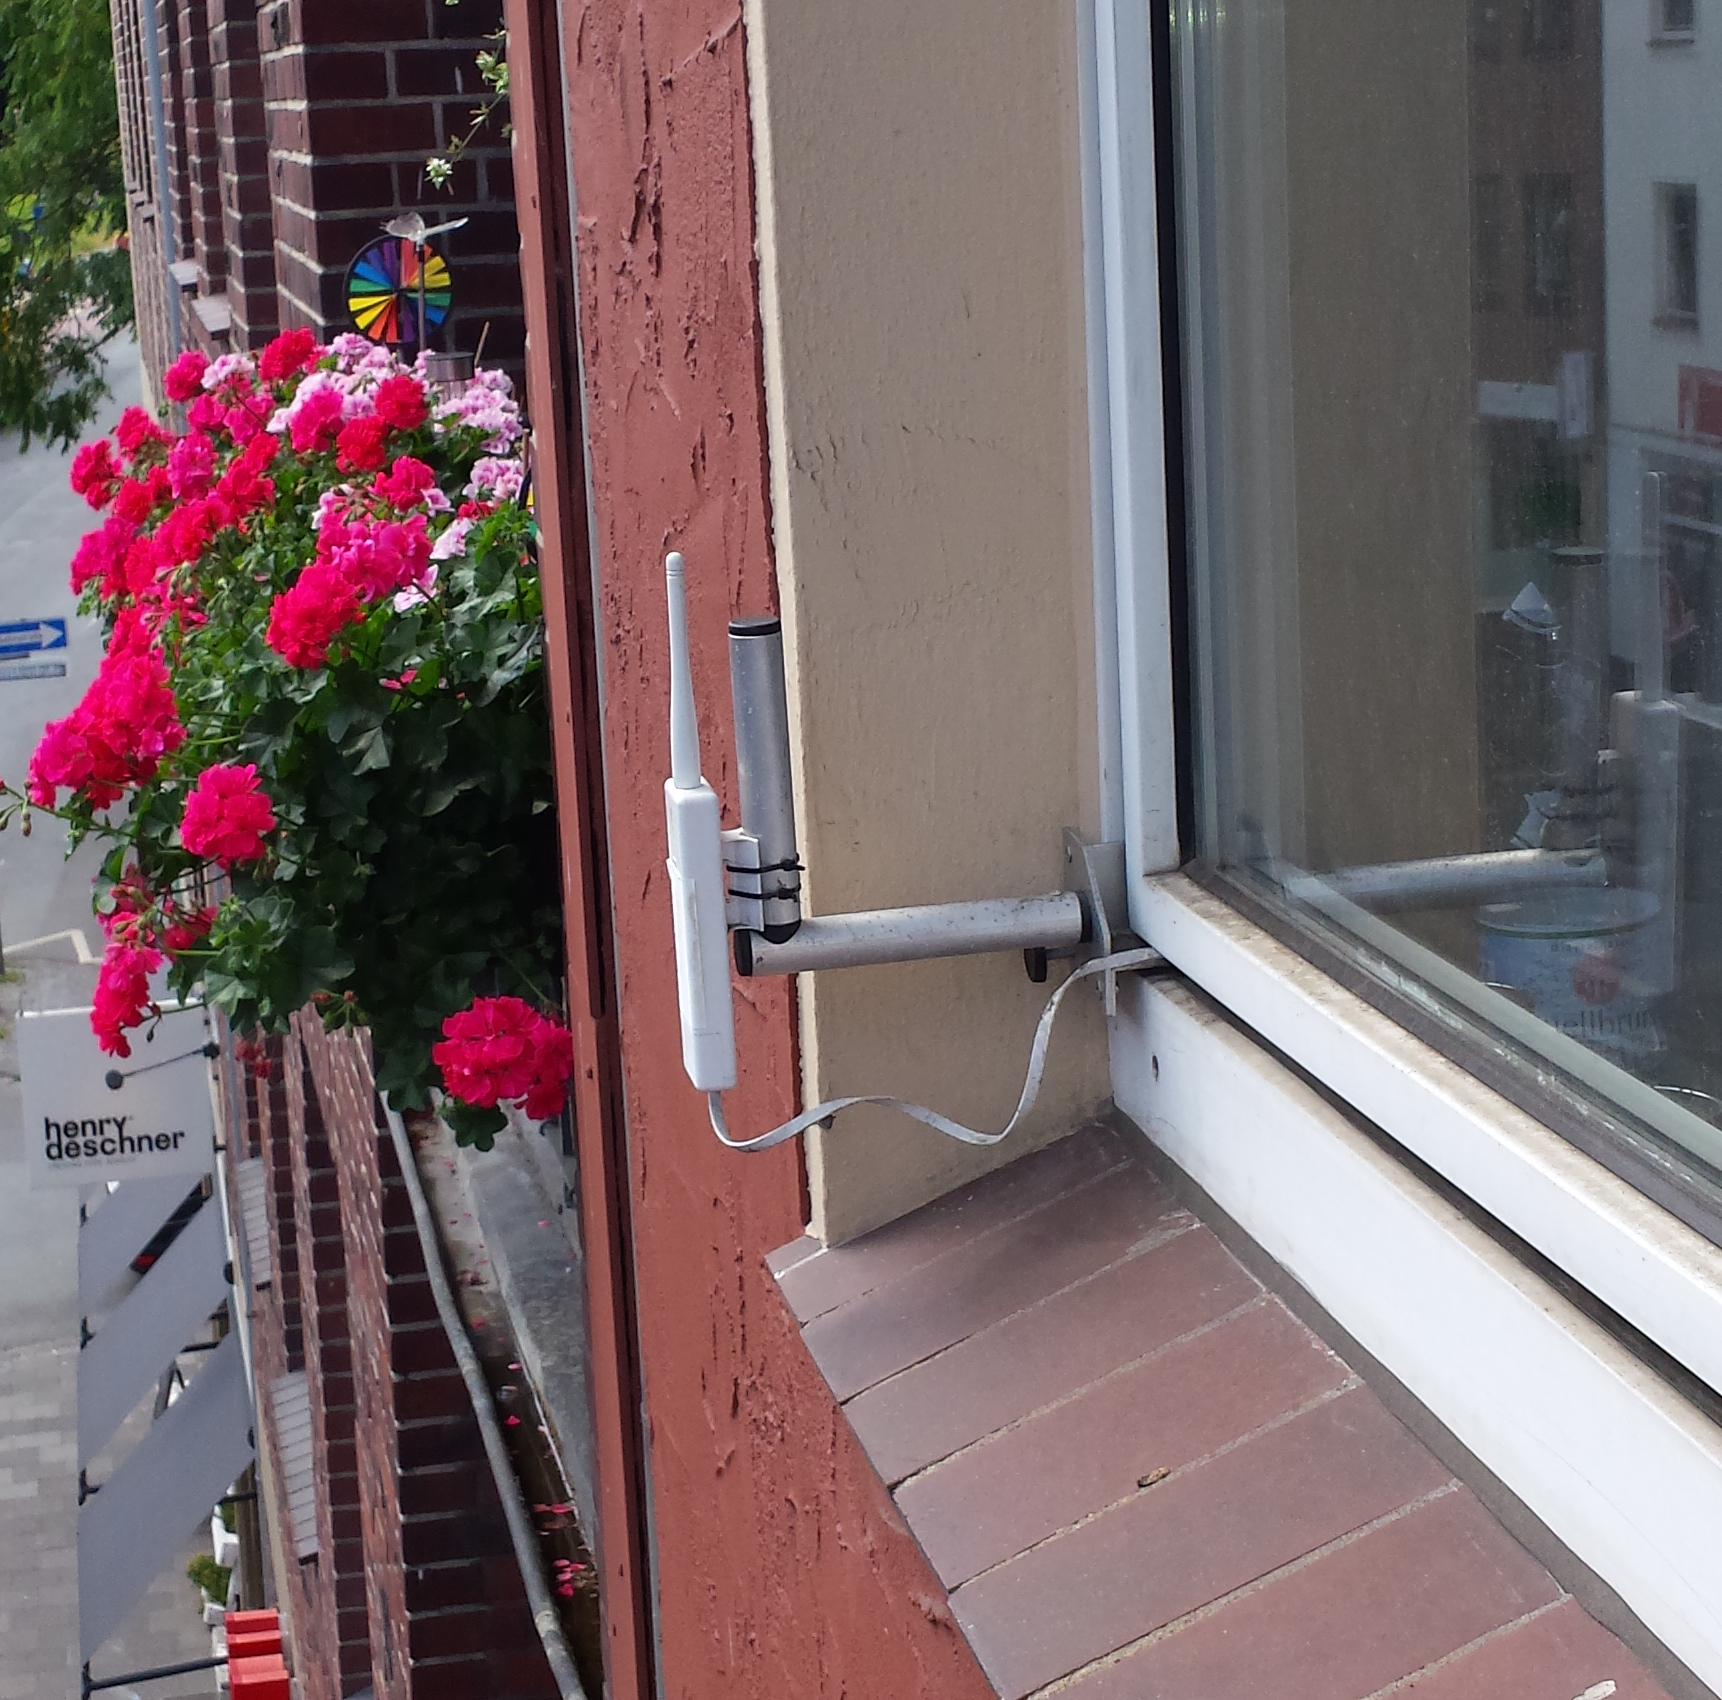
\includegraphics[height=0.5\textheight,keepaspectratio]{picostation.jpg}\\
			\vspace*{-2.0mm}\textit{\tiny Ubiquity Picostation}
			\begin{itemize}
				\item Rundstrahler
				\item ab 90 \euro
				\item Außengerät
			\end{itemize}
			
		\end{column}
	\end{columns}
\end{frame}
\subsection{Gemeinden}
\begin{frame}
	\begin{itemize}
		\item Zur Verfügungstellung von Glasfasern zur Vermaschung
	\end{itemize}
	\begin{center}
		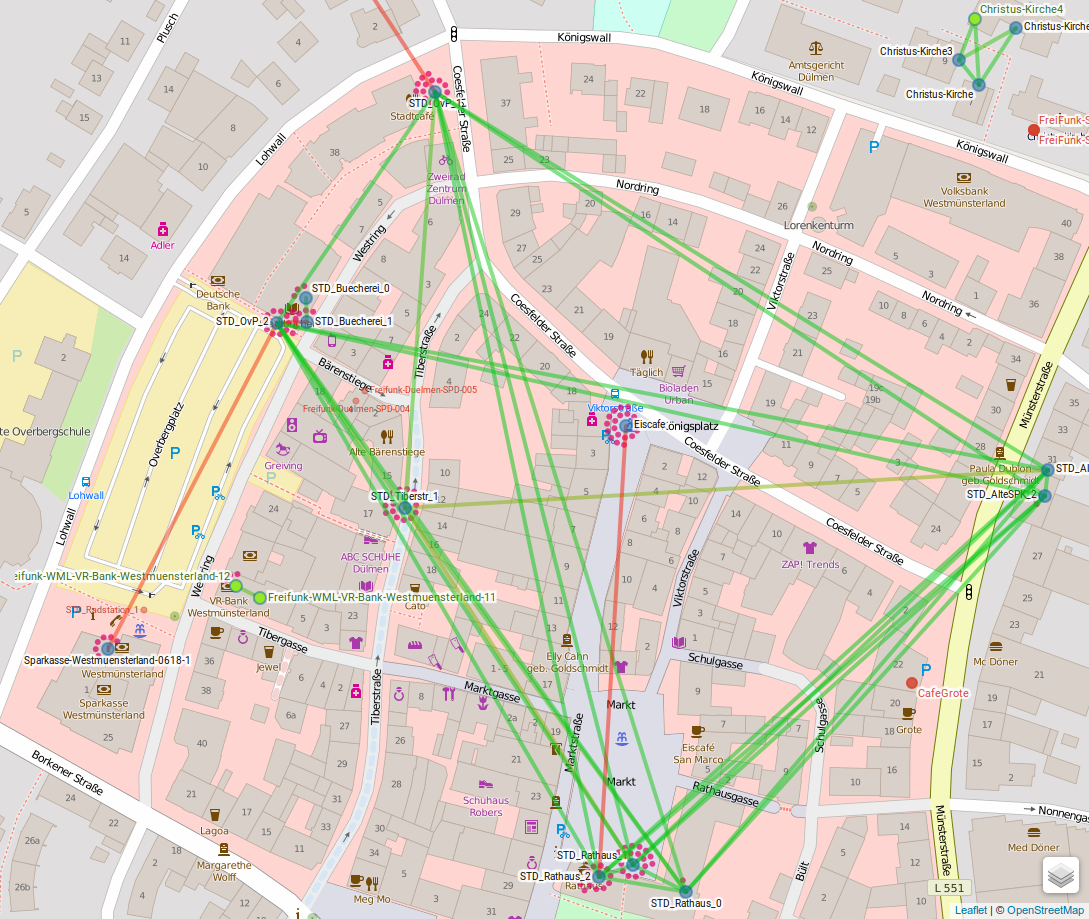
\includegraphics[height=0.8\textheight,keepaspectratio]{mesh-gemeinde.jpg}\\\vspace*{-2mm}\textit{\tiny\bigskip Dülmen}
	\end{center}
\end{frame}
\section{Kosten}
\begin{frame}{Was kostet Freifunk?}
	\begin{itemize}
		\item Stromkosten der Router (kleine Geräte ca. 5 \euro\ pro Jahr)
		\item Serverkosten
			\begin{itemize}
				\item derzeit 550 \euro\ pro Monat für das gesamte Münsterland
				\item Wird von Privatpersonen getragen
				\item Abwicklung zukünftig durch den Förderverein freie Infrastruktur e. V.
			\end{itemize}
		\item Wünschenswert: Geschäfte schließen Fördermitgliedschaft im FfI über 20 \euro\ pro Jahr ab
		\item Fördermitgliedschaftsantrag: {\tiny \href{https://github.com/ffimsl/Dokumente/raw/master/AntragFoerdermitgliedschaft.pdf}{https://github.com/ffimsl/Dokumente/raw/master/AntragFoerdermitgliedschaft.pdf}}
	\end{itemize}
\end{frame}
\begin{frame}
	\begin{center}
	\Huge Vielen Dank für's Zuhören
	\bigskip\\
	\ \bigskip\\
	Fragen?
	\end{center}
\end{frame}
\end{document}
